% !TEX program = xelatex
% Dream in Orbit : version publiable du rapport. Compilation : ./build.sh (XeLaTeX, via Tectonic ou latexmk).
% Les figures sont lues dans figures/ (produites par figures.py, voir README.md) ; la bibliographie est references.bib.
\documentclass[11pt,a4paper]{article}

% ---------- mathématiques et polices (XeLaTeX : fontspec + unicode-math) ----------
\usepackage{amsmath}
\usepackage{fontspec}
\usepackage{unicode-math}
\setmainfont{texgyrepagella}[
  Extension      = .otf,
  UprightFont    = *-regular,
  BoldFont       = *-bold,
  ItalicFont     = *-italic,
  BoldItalicFont = *-bolditalic]
\setmonofont{lmmono10-regular.otf}[
  BoldFont       = lmmonolt10-bold.otf,
  ItalicFont     = lmmono10-italic.otf,
  BoldItalicFont = lmmonolt10-boldoblique.otf,
  Scale          = MatchLowercase]
\setmathfont{texgyrepagella-math.otf}

% ---------- langue et typographie ----------
% Le français (dernière option) est la langue principale ; l'anglais sert à composer la bibliographie,
% pour que babel-french n'insère pas d'espace avant « : » dans les titres anglais et les identifiants.
\usepackage[english,french]{babel}
% babel-french nomme les tableaux « Table » : « Tableau » dans les légendes, comme dans les renvois (\autoref)
\addto\captionsfrench{\renewcommand{\tablename}{Tableau}}
\usepackage[autostyle=true,french=guillemets]{csquotes}
\usepackage[protrusion=true,expansion=false]{microtype}
\usepackage[a4paper,margin=2.5cm]{geometry}
\usepackage{booktabs}
\usepackage{tabularx}
\usepackage{graphicx}
\graphicspath{{figures/}}
\usepackage[labelfont=bf,font=small,labelsep=endash]{caption}
\usepackage{enumitem}
\setlist{itemsep=2pt,topsep=4pt,parsep=0pt}
\setlist[itemize]{label=\textendash}
\usepackage{xcolor}
\definecolor{lien}{RGB}{25,60,110}
\usepackage[numbers,sort&compress]{natbib}
\usepackage[colorlinks=true,linkcolor=lien,citecolor=lien,urlcolor=lien]{hyperref}
\hypersetup{pdftitle={Dream in Orbit : un world model de la consommation électrique de Mars Express},
            pdfauthor={Kenzi Lali},
            pdflang={fr}}
% noms des renvois \autoref en minuscules (« le tableau 3 », « la figure 2 »)
\addto\extrasfrench{%
  \def\tableautorefname{tableau}%
  \def\figureautorefname{figure}%
  \def\equationautorefname{équation}%
  \def\sectionautorefname{section}%
  \def\subsectionautorefname{section}%
}
% renvoi à une annexe (\autoref dirait « section A »)
\newcommand{\annexeref}[1]{\hyperref[#1]{annexe~\ref*{#1}}}

% placement des flottants un peu plus souple que les réglages par défaut
\setcounter{totalnumber}{4}
\renewcommand{\topfraction}{0.9}
\renewcommand{\bottomfraction}{0.8}
\renewcommand{\textfraction}{0.1}
\renewcommand{\floatpagefraction}{0.75}
% sur une page de flottants, les flottants commencent en haut et le blanc restant est en bas
\makeatletter
\setlength{\@fptop}{0pt}
\setlength{\@fpsep}{12pt plus 2pt}
\setlength{\@fpbot}{0pt plus 1fil}
\makeatother

% colonne tabularx en drapeau (fer à gauche)
\newcolumntype{Y}{>{\raggedright\arraybackslash}X}
% colonnes de largeur donnée, centrée ou en drapeau, dont le contenu peut se replier sur plusieurs lignes
\newcolumntype{C}[1]{>{\centering\arraybackslash}p{#1}}
\newcolumntype{L}[1]{>{\raggedright\arraybackslash}p{#1}}

\title{Dream in Orbit : un \emph{world model} de la consommation électrique de Mars Express}
% L'auteur peut ajuster ici son nom et, s'il le souhaite, ajouter une affiliation ou une adresse.
\author{Kenzi Lali}
\date{novembre 2026}

\begin{document}
\maketitle

\begin{abstract}
Nous simulons heure par heure, sur une année martienne entière (687~jours terrestres), la consommation électrique de 33~circuits de Mars Express à partir du planning, du contexte orbital et des 7~premiers jours réels. Le modèle final est un ensemble de cinq réseaux récurrents à portes (GRU) entraînés à rester stables sur 16\,000 pas de simulation libre (état caché transmis entre segments, \emph{scheduled sampling}), mélangé à parts égales avec un gradient boosting heure par heure. Trois validations chronologiques, dont une année de test qu'aucune décision de conception n'a vue, donnent une racine de l'erreur quadratique moyenne (RMSE) de 0,0750, 0,0901 et 0,0805, soit 23 à 29~\% de moins qu'une prédiction constante. Les ablations montrent que la physique (Soleil, pointage, saison) fait l'essentiel de la prédiction et que la procédure d'entraînement compte plus que l'architecture. Deux circuits de chauffage font 63~\% de l'erreur quadratique et changent de régime d'une année à l'autre pour des raisons que les données ne contiennent pas. L'incertitude de l'ensemble, calibrée par circuit d'une année de test sur l'autre, reste une échelle plutôt qu'une loi.
\end{abstract}

\section{Introduction}\label{sec:intro}

Mars Express est une sonde de l'Agence spatiale européenne (ESA) en orbite autour de Mars. Ce travail a été réalisé dans le cadre du défi étudiant Dream in Orbit, qui fournit un kit (deux années martiennes de télémétrie et de planning, un script qui construit une validation et un script d'évaluation) ; le jeu de test final, tenu par les organisateurs, est l'année martienne suivante. Les deux périodes du kit, \texttt{annee1} et \texttt{annee2}, couvrent chacune 687~jours terrestres, soit une année martienne, et se suivent (du 22~août 2008 au 9~juillet 2010, puis du 10~juillet 2010 au 26~mai 2012). Les six fichiers du kit (télémétrie de puissance, commandes, pointages, angles solaires, événements orbitaux, tendances journalières) semblent reprendre, aux noms de fichiers près, le format, les colonnes et les deux premières années martiennes du jeu de données publié par l'ESA pour le Mars Express Power Challenge de 2016 \citep{esa2016kelvins,lucas2017mars}, dont l'objet était déjà de prédire la consommation du sous-système thermique sur l'année martienne suivante \citep{petkovic2019machine} ; le kit lui-même n'indique pas sa provenance.

La tâche est de simuler, heure par heure et sur toute la période de test, la consommation de 33~circuits (NPWDxxxx) à partir du planning (commandes, pointages), du contexte (angles solaires, événements, tendances journalières) et des 7~premiers jours réels. La métrique est la racine de l'erreur quadratique moyenne (RMSE) de simulation, définie par l'\autoref{eq:rmse} (\autoref{sec:protocole}) et calculée par le script d'évaluation du kit. Les valeurs sont en unités du fichier de télémétrie (courants électriques moyens par circuit ; le kit ne précise pas l'unité) et la RMSE s'exprime dans la même unité.

\paragraph{\emph{World model} et travaux connexes.}
Le terme de world model vient de l'apprentissage par renforcement : Ha et Schmidhuber \citep{ha2018world}, puis Hafner et al. \citep{hafner2019planet,hafner2020dream}, apprennent un modèle de la dynamique d'un environnement et l'utilisent pour \enquote{rêver}, c'est-à-dire simuler des trajectoires entières en se nourrissant de leurs propres prédictions. Ici l'environnement est la sonde, les actions sont le planning, le contexte est la physique orbitale et l'état est la consommation des 33~circuits. Avec les notations de la \autoref{sec:modele}, le modèle apprend
\begin{equation*}
  (y_{t-1},\, x_t) \;\longmapsto\; y_t ,
\end{equation*}
où $y_t$ est la consommation des 33~circuits à l'heure $t$ et $x_t$ regroupe les actions et le contexte de la même heure. Après les 7~jours réels, le modèle réinjecte sa propre prédiction comme état précédent : c'est la situation exacte de l'évaluation, et c'est ce que l'entraînement doit préparer. Un modèle récurrent entraîné à prédire le pas suivant mais évalué en simulation libre souffre du biais d'exposition : le \emph{scheduled sampling} \citep{bengio2015scheduled} l'expose à ses propres sorties pendant l'entraînement, au prix d'un objectif qui n'est plus celui de la vraisemblance \citep{huszar2015hownot}. Le Mars Express Power Challenge posait un problème voisin : prédire la consommation du sous-système thermique sur une année martienne à partir du planning et du contexte des années précédentes \citep{lucas2017mars}. Les solutions décrites par Petković et al. \citep{petkovic2019machine} reposent sur des features construites à la main à partir des mêmes fichiers (commandes, pointages, angles solaires, événements) et sur des ensembles d'arbres (gradient boosting, forêts aléatoires), chaque heure étant prédite à partir du seul contexte de l'heure. Le présent travail se situe entre ces deux familles : une régression contextuelle sur les mêmes entrées que les solutions du concours, mais sous une contrainte de stabilité sur 16\,000 pas de simulation libre, avec un mélange d'un réseau récurrent et d'arbres, et des ablations qui mesurent ce que chaque ingrédient vaut.

\paragraph{Contributions.}
\begin{itemize}
  \item un jeu de features (variables d'entrée) construit \emph{sans lettre de variante} de commande, après la découverte que ces lettres changent d'une année martienne à l'autre pour 20 des 29 interrupteurs, et un protocole d'évaluation en trois validations chronologiques, dont une année de test qu'aucune décision de conception n'a vue (\autoref{sec:donnees} et \autoref{sec:protocole}) ;
  \item un modèle hybride, ensemble de réseaux récurrents à portes (GRU) \citep{cho2014gru} entraîné pour la simulation libre et mélangé à parts égales avec un composant gradient boosting en \emph{bagging} temporel, qui bat chacune de ses composantes dans les trois protocoles, avec 0,0750, 0,0901 et 0,0805 de RMSE (\autoref{sec:modele} et \autoref{sec:resultats}) ;
  \item une analyse de l'erreur qui en ramène 63~\% à deux circuits de chauffage et 60~\% à 1,5~\% des cellules, avec le diagnostic du décrochage de 2011 et une borne (la RMSE plancher avec ces entrées est vers 0,071), et des ablations qui situent chaque ingrédient : la physique d'abord, la procédure d'entraînement avant l'architecture, des ajouts qui nuisent (\autoref{sec:erreurs} et \autoref{sec:ablations}) ;
  \item une incertitude calibrée par circuit et vérifiée d'une année de test sur l'autre, et une application de pilotage qui compare des plannings alternatifs en comparaison appariée (\autoref{sec:resultats} et \autoref{sec:pilote}).
\end{itemize}
Le journal des essais, négatifs compris, et les commandes qui reproduisent tout le rapport sont en annexe (\annexeref{app:journal} et \annexeref{app:repro}).

\section{Données}\label{sec:donnees}

Tout est aligné sur une grille horaire calendaire : une ligne par heure UTC, du premier au dernier début d'heure de la période, soit 16\,488 heures par période de 687~jours. La vérité est la moyenne horaire des mesures de la télémétrie de puissance, calculée exactement comme le script de validation du kit ; la télémétrie couvre 16\,456 de ces heures pour \texttt{annee1} et 16\,242 pour \texttt{annee2}, et les heures sans aucune mesure (32 dans \texttt{annee1}, en dix trous d'au plus 7\,h ; 246 dans \texttt{annee2}, en 47 trous d'au plus 22\,h, dont une série entre le 13 et le 30~août 2011, juste avant le trou de commandes du 30~août) sont ignorées dans la perte comme dans le score : en strict, 16\,073 heures sont notées sur les 16\,319 prédites. Le \autoref{tab:kit} résume les six fichiers du kit ; les fiches détaillées (format, vocabulaire, préfixes de colonnes, liens physiques) sont en \annexeref{app:fiches}.

\begin{table}[htbp]
\centering\footnotesize
\caption{Les six fichiers du kit : rôle, volume (\texttt{annee1} / \texttt{annee2}), features dérivées et piège principal. Le détail de chaque fichier est en annexe~\ref{app:fiches}, tableaux \ref{tab:power} à \ref{tab:ltdata}.}
\label{tab:kit}
\begin{tabularx}{\textwidth}{L{2.7cm} L{2.4cm} Y Y}
\toprule
Fichier (rôle) & Lignes & Features dérivées & Piège \\
\midrule
\textbf{power.csv} : l'état, 33~circuits NPWDxxxx (courant moyen par circuit, de 0 à $\approx$\,2,2) & 1,83 million / 1,77 million (une mesure toutes les $\approx$\,32\,s) & la cible : moyenne horaire par circuit ; 13 à 17 circuits selon l'année sont quasi constants & changements de régime d'une année à l'autre ; deux lignes de chauffage à thermostat (NPWD2551, NPWD2451) font 61~\% de l'erreur quadratique de la constante \\
\textbf{dmop.csv} : les commandes (actions) & 187\,000 / 144\,000 & comptes horaires par stem (commande sans sa lettre de variante), commandes à venir à 1\,h et à 6\,h, heures depuis et jusqu'au prochain changement de variante, comptes et récences par sous-système, intervalles début/fin & les lettres de variante changent d'une année à l'autre (20 interrupteurs sur 29) ; un sous-système (AACF) n'existe que dans \texttt{annee2} ; trous de 34 et 35~jours \\
\textbf{ftl.csv} : les pointages (actions) & 19\,600 / 20\,000 intervalles & fraction d'heure par type de pointage (16 types), fraction avec communication, changements de pointage dans l'heure & le mode D4PNPO couvre 658\,h d'\texttt{annee1} et 1\,958\,h d'\texttt{annee2} \\
\textbf{saaf.csv} : les angles du Soleil (contexte) & 1,26 million / 1,31 million (toutes les $\approx$\,47\,s) & moyennes horaires des quatre angles et de leurs cosinus, écart-type horaire de l'aspect solaire & l'ingrédient n\textsuperscript{o}\,1 (ablation : +0,020) ; trous comblés par interpolation \\
\textbf{evtf.csv} : les événements orbitaux (contexte) & 76\,800 / 75\,200 & fractions d'heure en ombre, en occultation, en contact station ; temps depuis et jusqu'au péricentre, phase orbitale, altitude & presque redondant avec les angles solaires et les durées d'éclipse (ablation : +0,001) \\
\textbf{ltdata.csv} : les tendances journalières (contexte) & 687 / 687 (une par jour) & interpolation horaire des distances, de l'angle Soleil-Mars-Terre, de la constante solaire, des durées d'éclipse et d'occultation & distance Terre-Mars et angle Soleil-Mars-Terre sont un calendrier déguisé : retirés (ablation : +0,009) \\
\bottomrule
\end{tabularx}
\end{table}

\paragraph{L'état.} La télémétrie de puissance des 33~circuits est la grandeur à simuler ; six circuits font l'essentiel de l'erreur quadratique d'une prédiction constante, et deux d'entre eux, NPWD2551 et NPWD2451, sont des lignes de chauffage à thermostat : fortes pendant les saisons d'éclipses (moyenne 0,5--0,8 contre 0,03--0,1 hors saison), avec des cycles ON/OFF à l'échelle de l'orbite (7\,h) et une autocorrélation à 1\,h de 0,6 seulement. Leur régime change d'une année à l'autre : NPWD2551 s'éteint en janvier 2011 malgré les éclipses, décroche le 30~août 2011 (\autoref{sec:erreurs}) et s'allume en février--mars 2012 sans éclipse.

\paragraph{Les actions.} Les commandes sont nommées par quatre lettres de sous-système, un code et une lettre de variante. Ce vocabulaire dérive d'une année à l'autre : sur les deux années réunies, 29~interrupteurs (stems à plusieurs variantes fréquentes) sont observés, dont 18 dans le vocabulaire appris sur \texttt{annee1}, et les lettres de variante changent pour 20 d'entre eux ; un sous-système entier n'existe que dans \texttt{annee2} ; et le fichier contient des trous de plusieurs semaines. Les features retenues sont donc construites \emph{sans lettre de variante} : comptes horaires par stem, commandes à venir, changements de variante à venir et passés. Les pointages donnent, par intervalle, l'attitude de la sonde et un drapeau de communication ; l'attitude décide quelle face reçoit le Soleil, et c'est l'un des ingrédients les plus utiles (\autoref{sec:ablations}).

\paragraph{Le contexte.} Les angles entre la direction du Soleil et les axes de la sonde sont l'ingrédient numéro un du modèle : moins de Soleil sur la face chauffée, plus de chauffage. Les événements orbitaux (ombres, occultations, passages au péricentre et à l'apocentre, contacts avec les stations sol) sont résumés en fractions d'heure et en phase orbitale. Les tendances journalières (distances, angle Soleil-Mars-Terre, constante solaire, durées d'éclipse et d'occultation) sont interpolées à l'heure ; deux de ces colonnes, la distance Terre-Mars et l'angle Soleil-Mars-Terre, jouent le rôle de calendrier, parce que leur période (780~jours) diffère de l'année martienne (687~jours) : le couple (distance Soleil-Mars, distance Terre-Mars), de périodes 687 et 780~jours, identifie la date de façon unique. Un réseau les utilise pour mémoriser l'année d'entraînement : nous les retirons (ablation : +0,009, \autoref{tab:ablations}).

\section{Protocole d'évaluation}\label{sec:protocole}

Trois validations, toujours chronologiques, jamais aléatoires, toutes sous la forme exacte de l'évaluation : 7~jours réels, puis simulation libre de tout le reste (\autoref{tab:protocoles}). La RMSE de simulation est
\begin{equation}\label{eq:rmse}
  \mathrm{RMSE} = \sqrt{\frac{1}{\lvert C\rvert}\sum_{(t,c)\in C}\bigl(\hat{y}_{t,c}-y_{t,c}\bigr)^2},
\end{equation}
où $C$ est l'ensemble des cellules (heure $t$, circuit $c$) de la période de test après les 7~premiers jours pour lesquelles la vérité existe, $y_{t,c}$ la moyenne horaire mesurée et $\hat{y}_{t,c}$ la valeur simulée (530\,409 cellules en protocole strict) ; les 33~circuits pèsent à égalité quelle que soit leur amplitude, ce qui explique que deux circuits puissent faire 63~\% de l'erreur quadratique (\autoref{sec:erreurs}). C'est la définition du script d'évaluation du kit (moyenne sur toutes les cellules où la vérité existe), que la fonction de métrique du dépôt reproduit.

\begin{table}[htbp]
\centering\small
\caption{Les trois protocoles de validation. Chacun entraîne sur une période, puis simule librement la période de test après ses 7~premiers jours réels.}
\label{tab:protocoles}
\begin{tabularx}{\textwidth}{l l l Y}
\toprule
Protocole & Entraînement & Test & Ce qu'il mesure \\
\midrule
\textbf{strict} & \texttt{annee1} & \texttt{annee2} (16\,242\,h) & une année nouvelle, avec de nouvelles lettres de commandes et de nouveaux régimes : le cas de l'évaluation finale \\
\textbf{inversé} & \texttt{annee2} & \texttt{annee1} & la même chose dans l'autre sens, sur une année de test qu'\textbf{aucune} décision de conception n'a vue \\
\textbf{chronologique} & \texttt{annee1} + $\tfrac{1}{2}$~\texttt{annee2} & $\tfrac{1}{2}$~\texttt{annee2} (8\,121\,h) & deux ans d'entraînement, lettres de commandes stables : ce que le modèle gagne à connaître le vocabulaire de l'année testée \\
\bottomrule
\end{tabularx}
\end{table}

Deux règles d'hygiène. \textbf{Le vocabulaire des features est appris sur la période d'entraînement seule} (noms des stems, interrupteurs, types de pointage ; en chronologique, à la date de coupure) : rien de la période de test n'entre dans la définition des colonnes, comme au test final où le vocabulaire vient des métadonnées du modèle final. Et \textbf{le protocole inversé a été ajouté après toutes les décisions} (features, hyperparamètres, poids de mélange, nombre de sacs, toutes prises sur strict et chronologique) : il mesure l'optimisme de sélection, inévitable quand une seule année de test sert à des dizaines de choix. Le bruit entre graines est de $\pm$\,0,001 sur la RMSE d'un GRU seul : un écart inférieur à 0,002 n'est pas significatif.

Repères (RMSE de références naïves) : constante = 0,1058 (strict), 0,1252 (inversé), 0,1048 (chronologique) ; constante calée sur les 7~premiers jours = 0,1116 / 0,1494 / 0,1269 ; persistance de la dernière heure = 0,1378 / 0,1689 / 0,1416 ; gradient boosting heure par heure sans mémoire, sur toutes les colonnes (\texttt{baselines.py}, référence distincte du composant GBM du modèle) = 0,1055 / non mesuré / 0,0998.

\section{Modèle}\label{sec:modele}

Soit $x_t$ le vecteur des features de l'heure $t$ (contexte et planning, 162 colonnes standardisées en protocole strict) et $y_{t-1}$ la consommation de l'heure précédente (33~circuits, standardisés). Chaque GRU de l'ensemble s'écrit
\begin{align}
  h_t &= \mathrm{GRU}\bigl(h_{t-1},\, \phi([x_t,\, y_{t-1}])\bigr)
      && \text{mémoire : état caché (128)} \label{eq:gru}\\
  \hat{y}^{\mathrm{GRU}}_t &= \psi(h_t)
      && \text{tête : 33 sorties} \label{eq:tete}
\end{align}
et la prédiction finale est le mélange
\begin{equation}
  \hat{y}_t = 0{,}5\,\overline{\hat{y}^{\mathrm{GRU}}_t} + 0{,}5\,\mathrm{GBM}\bigl(x^{\mathrm{GBM}}_t\bigr), \label{eq:melange}
\end{equation}
où GRU est une unité récurrente à portes \citep{cho2014gru}, $\phi$ une couche linéaire $195 \to 128$ en strict ($162 + 33$ entrées) suivie d'une GELU (\emph{Gaussian Error Linear Unit}), $\psi$ un perceptron multicouche (MLP) $128 \to 128 \to 33$, $\overline{\hat{y}^{\mathrm{GRU}}_t}$ la moyenne des cinq GRU (cinq graines) et $x^{\mathrm{GBM}}_t$ le vecteur de features, plus large (684 colonnes en strict), lu par le composant gradient boosting (GBM, \emph{gradient boosting machine} \citep{friedman2001greedy}). La perte d'un GRU est l'erreur quadratique moyenne (MSE) sur l'échelle brute. Nous appelons \emph{membre} de l'ensemble un GRU (une graine) mélangé au GBM selon l'\autoref{eq:melange} : la prédiction finale est la moyenne des cinq membres, et leur écart-type sert d'incertitude. Le \autoref{tab:hyper} rassemble les hyperparamètres ; les dimensions sont celles du protocole strict, le modèle final, entraîné sur les deux années avec un vocabulaire plus large, lisant 196 features dans le GRU ($\phi : 229 \to 128$) et 846 colonnes dans le GBM.

\begin{table}[htbp]
\centering\small
\caption{Hyperparamètres du système (dimensions du protocole strict ; le modèle final, entraîné sur les deux années, lit 196 features dans le GRU et 846 colonnes dans le GBM).}
\label{tab:hyper}
\begin{tabularx}{\textwidth}{L{3.4cm} Y}
\toprule
Ensemble de GRU & état caché 128, une couche ; entrée $\phi$ : couche linéaire $195 \to 128$ (strict) et GELU ; tête $\psi$ : $128 \to 128 \to 33$ avec GELU ; 16 flux contigus, segments de 168\,h ; 80 époques dont 15 en teacher forcing, puis scheduled sampling jusqu'à $p = 0$ ; AdamW \citep{loshchilov2019decoupled} (taux $10^{-3}$, weight decay $10^{-3}$) et OneCycle \citep{smith2017super} ; dropout 0,3, dropout de features 0,2, bruit 0,05 sur l'état réinjecté ; perte MSE sur l'échelle brute ; 5 graines \\
Composant gradient boosting & un \texttt{HistGradientBoostingRegressor} de scikit-learn par circuit : 600 arbres, taux d'apprentissage 0,02, 15 feuilles, 100 observations par feuille, $\ell_2 = 3$ ; 684 colonnes (strict) ; bagging temporel en 5 sacs \\
Mélange et incertitude & $0{,}5 \times$ moyenne des cinq GRU $+\ 0{,}5 \times$ GBM ; écart-type des cinq membres, multiplié par un facteur par circuit (\autoref{sec:incertitude}) \\
\bottomrule
\end{tabularx}
\end{table}

\paragraph{Entrées du GRU.} Cinq groupes de features, un par fichier de contexte ou de planning, composent $x_t$ : angles solaires et leurs cosinus ; ombres, occultations, phase orbitale et altitude ; pointage (fraction par type, communication) ; constante solaire et durées d'éclipse et d'occultation ; comptes horaires de commandes par stem, sans lettre de variante. Pas de calendrier (distance Terre-Mars, angle Soleil-Mars-Terre), pas de récences (\enquote{heures depuis\ldots} : des rampes de plusieurs semaines qui servent d'horloge au réseau, \annexeref{app:journal}).

\paragraph{Entraînement par flux continus.} La période est découpée en 16 flux contigus ; nous avançons par segments de 168\,h en transmettant l'état caché $h_t$ de l'\autoref{eq:gru} d'un segment au suivant (rétropropagation dans le temps tronquée, BPTT), avec un décalage aléatoire à chaque époque : c'est l'entraînement \emph{stateful}, qui place le réseau dans les conditions de la simulation longue. Scheduled sampling \citep{bengio2015scheduled} : 15 époques en \emph{teacher forcing} \citep{williams1989learning}, où la vérité est réinjectée comme état précédent, puis la probabilité de réinjecter la vérité décroît vers 0 ; un bruit gaussien (0,05 en unités standardisées) est ajouté à l'état réinjecté.

\paragraph{Composant gradient boosting.} Un \texttt{HistGradientBoostingRegressor} de scikit-learn \citep{pedregosa2011scikit}, dans l'esprit de LightGBM \citep{ke2017lightgbm}, par circuit, sur toutes les colonnes sauf les calendriers, les statistiques glissantes et toute feature encodée par lettre ; \textbf{bagging temporel en 5 sacs} \citep{breiman1996bagging}, chaque sac entraîné sans un bloc contigu d'un cinquième de la période, prédiction = moyenne des sacs. Déterministe, sans mémoire, aveugle aux 7~jours réels.

\paragraph{Mélange à parts égales.} Le poids 0,5 a été choisi sur les protocoles strict et chronologique avant l'existence du protocole inversé (\autoref{sec:resultats}).\footnote{Le règlement du défi n'admet les modèles classiques que comme référence ou comme composant : le modèle final est un réseau de neurones (l'ensemble de GRU) auquel un composant gradient boosting est adjoint dans un mélange à parts égales. Sans ce composant, l'ensemble de GRU seul donne 0,0796 en strict ; avec un poids de 0,3 pour le GBM, 0,0758.} L'empilement (le GRU lit la prédiction hors-échantillon du GBM et apprend à la corriger) a été essayé et nettement battu par le mélange (0,0908 contre 0,0751 à une graine, en strict) : les prédictions hors-échantillon des sacs sont des erreurs d'extrapolation de saison (un sac n'a jamais vu d'éclipses) qui ne ressemblent pas aux erreurs du GBM complet au test ; le GRU apprend à corriger des erreurs qui n'existent plus.

\paragraph{Incertitude.} L'écart-type des cinq prédictions finales (\emph{Deep Ensembles} \citep{lakshminarayanan2017deep}), multiplié par un facteur par circuit ajusté sur une année de validation et vérifié sur l'autre ; la calibration et la couverture sont mesurées à la \autoref{sec:incertitude}.

\section{Résultats}\label{sec:resultats}

Tous les chiffres de cette section et des suivantes sont produits par les scripts du dépôt (\annexeref{app:repro}). Le \autoref{tab:resultats} donne la RMSE de simulation (7~jours réels puis rêve sur toute la période) du système final et de ses composantes dans les trois protocoles.

\begin{table}[htbp]
\centering\small
\caption{RMSE de simulation dans les trois protocoles : références, composantes seules et world model final. La dernière ligne est la réduction du world model par rapport à la constante.}
\label{tab:resultats}
\begin{tabularx}{\textwidth}{Y C{3cm} C{3cm} C{3.2cm}}
\toprule
Modèle & strict & inversé & chronologique \\
 & \texttt{annee1} $\rightarrow$ \texttt{annee2} & \texttt{annee2} $\rightarrow$ \texttt{annee1} & 2 ans $\rightarrow$ $\tfrac{1}{2}$~\texttt{annee2} \\
\midrule
Constante (moyenne de la période d'entraînement) & 0,1058 & 0,1252 & 0,1048 \\
Gradient boosting seul (5 sacs, sans lettre) & 0,0792 & 0,0908 & 0,0816 \\
Ensemble de GRU seul (5 graines ; 3 en chronologique) & 0,0796 & 0,0952 & 0,0884 \\
\textbf{World model final : 0,5 GRU + 0,5 GBM} & \textbf{0,0750} & \textbf{0,0901} & \textbf{0,0805} \\
\midrule
réduction par rapport à la constante & 29~\% & 28~\% & 23~\% \\
\bottomrule
\end{tabularx}
\end{table}

Le flux officiel du kit (construction de la validation, prédiction, évaluation), avec le modèle entraîné sur \texttt{annee1} seule, donne 0,074968 sur 530\,409 cellules notées. Les cinq membres de l'ensemble strict (un GRU par graine, chacun mélangé au GBM) sont entre 0,0749 et 0,0763 ; les moyenner gagne peu : les erreurs restantes sont systématiques, pas du bruit de graine. Le protocole inversé, qui n'a servi à aucun choix, donne une réduction du même ordre que le strict : l'optimisme de sélection sur le strict est au plus de quelques millièmes.

Le \autoref{tab:poids} donne la RMSE du mélange pour chaque poids du GBM. Les écarts entre 0,5 et 0,7 (au plus 0,0007) sont inférieurs au seuil de 0,002 de la \autoref{sec:protocole} ; 0,5 a été choisi sur les protocoles strict et chronologique, et la ligne inversée est une vérification \emph{a posteriori}.

\begin{table}[htbp]
\centering\small
\caption{RMSE du mélange selon le poids du composant gradient boosting (le complément est le poids de l'ensemble de GRU). Le poids final, 0,5, a été choisi sur les protocoles strict et chronologique ; la ligne inversée est une vérification \emph{a posteriori}.}
\label{tab:poids}
\begin{tabular}{l c c c c c}
\toprule
poids du GBM & 0,3 & 0,4 & \textbf{0,5} & 0,6 & 0,7 \\
\midrule
strict & 0,0758 & 0,0752 & \textbf{0,0750} & 0,0751 & 0,0756 \\
inversé & 0,0915 & 0,0907 & \textbf{0,0901} & 0,0898 & 0,0897 \\
chronologique & 0,0826 & 0,0814 & \textbf{0,0805} & 0,0799 & 0,0798 \\
\bottomrule
\end{tabular}
\end{table}

\subsection{Erreur par circuit}\label{sec:circuits}

Le \autoref{tab:circuits} (protocole strict) détaille les sept circuits qui pèsent le plus. Deux circuits font 63~\% de l'erreur quadratique ; sur chacun, le mélange bat ses deux composantes. Les erreurs du GRU et du GBM ne sont corrélées qu'à 0,78 : c'est pour cela que leur moyenne gagne, alors que deux GRU de graines différentes sont corrélés à 0,96--0,99.

\begin{table}[htbp]
\centering\small
\caption{Erreur par circuit en protocole strict (\texttt{annee2} en test) : RMSE du système final, de l'ensemble de GRU seul et du GBM seul, écart-type réel du circuit et part de l'erreur quadratique totale.}
\label{tab:circuits}
\begin{tabular}{l c c c c c}
\toprule
Circuit & système final & GRU seul & GBM seul & écart-type réel & part de l'erreur quadratique \\
\midrule
NPWD2551 & 0,261 & 0,282 & 0,279 & 0,366 & 37~\% \\
NPWD2451 & 0,221 & 0,237 & 0,228 & 0,299 & 26~\% \\
NPWD2532 & 0,129 & 0,141 & 0,125 & 0,158 & 9~\% \\
NPWD2851 & 0,124 & 0,118 & 0,149 & 0,136 & 8~\% \\
NPWD2881 & 0,083 & 0,092 & 0,087 & 0,122 & 4~\% \\
NPWD2561 & 0,082 & 0,090 & 0,087 & 0,120 & 4~\% \\
NPWD2531 & 0,078 & 0,075 & 0,093 & 0,081 & 3~\% \\
\bottomrule
\end{tabular}
\end{table}

\subsection{Courbe de dérive}\label{sec:derive}

La \autoref{fig:derive} trace la RMSE de chaque semaine depuis le début du rêve ; le \autoref{tab:derive} la résume par horizon.

\begin{table}[htbp]
\centering\small
\caption{RMSE moyenne des semaines selon l'horizon depuis le début du rêve (protocole strict, 98 semaines, numérotées à partir de 1).}
\label{tab:derive}
\begin{tabular}{l c}
\toprule
Horizon depuis le début du rêve & RMSE moyenne des semaines \\
\midrule
semaines 1--4 & 0,039 \\
semaines 5--50 & 0,064 \\
semaines 51--98 & 0,083 \\
\bottomrule
\end{tabular}
\end{table}

\begin{figure}[htbp]
\centering
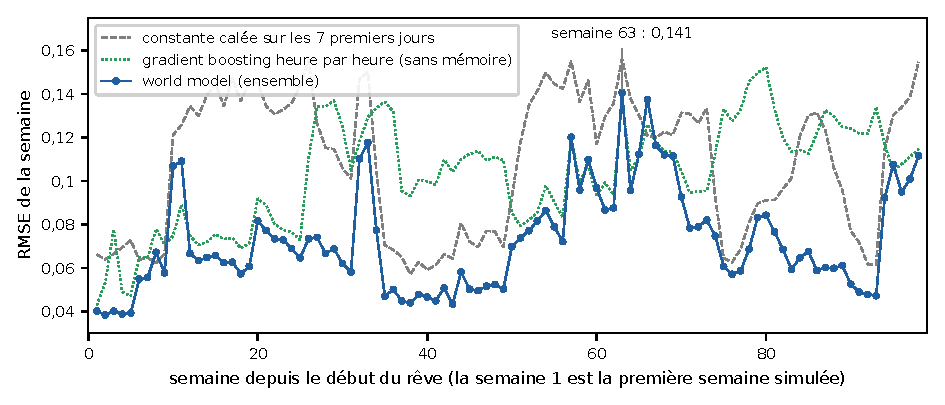
\includegraphics[width=\textwidth]{derive.pdf}
\caption{Courbe de dérive en protocole strict (\texttt{annee2}) : RMSE de chaque semaine depuis le début du rêve pour le world model (ensemble), pour la constante calée sur les 7~premiers jours et pour la référence gradient boosting heure par heure de \texttt{baselines.py} (toutes les colonnes, lettres comprises ; RMSE 0,1055 en strict, \autoref{sec:protocole}), distincte du composant GBM du modèle final (0,0792). Les semaines sont numérotées à partir de 1, comme dans le texte et le \autoref{tab:derive} ; la pire semaine (63, RMSE 0,141) est annotée. L'erreur ne croît pas avec l'horizon : elle suit les saisons d'éclipses.}
\label{fig:derive}
\end{figure}

L'erreur ne s'accumule pas avec l'horizon : elle suit les saisons (pics pendant les deux saisons d'éclipses, où la constante et le gradient boosting de référence montent à 0,13--0,15). La pire semaine (semaine 63, 0,141) est dans la deuxième saison d'éclipses de 2011, au décrochage de NPWD2551 (\autoref{sec:erreurs}). Le mécanisme anti-dérive est double : état caché entraîné sur des flux longs, et apprentissage sur ses propres prédictions (scheduled sampling jusqu'à $p = 0$).

\subsection{Incertitude : calibration et couverture}\label{sec:incertitude}

L'écart-type brut de l'ensemble suit l'erreur (corrélation de Spearman 0,82 entre écart-type et erreur absolue) mais il est sous-dispersé d'un facteur 11 : il classe les heures incertaines, il ne les quantifie pas. Les facteurs par circuit sont ajustés sur le protocole inversé (\texttt{annee1} en test), puis appliqués tels quels aux deux autres (\autoref{tab:calibration}).

\begin{table}[htbp]
\centering\small
\caption{Couverture des intervalles de l'ensemble avant et après calibration, et rapport entre la RMSE et la moyenne quadratique de l'écart-type calibré. Les facteurs par circuit sont ajustés sur le protocole inversé et transférés tels quels aux deux autres ; attendu sous une loi gaussienne : 68~\% à $\pm 1\sigma$ et 95~\% à $\pm 2\sigma$.}
\label{tab:calibration}
\begin{tabularx}{\textwidth}{Y C{1.7cm} C{1.7cm} C{1.7cm} C{1.7cm} C{2.8cm}}
\toprule
 & \multicolumn{4}{c}{couverture} & \\
\cmidrule(lr){2-5}
protocole (test) & $\pm 1\sigma$ brute & $\pm 2\sigma$ brute & $\pm 1\sigma$ calibrée & $\pm 2\sigma$ calibrée & RMSE / RMS($\sigma$) calibré \\
\midrule
strict (\texttt{annee2}) & 13~\% & 22~\% & 45~\% & 64~\% & 1,63 \\
chronologique ($\tfrac{1}{2}$~\texttt{annee2}) & 11~\% & 18~\% & 38~\% & 57~\% & 1,64 \\
inversé (\texttt{annee1}, ajustement) & --- & --- & 60~\% & 81~\% & 1,00 \\
\bottomrule
\end{tabularx}
\end{table}

Les facteurs transférés d'une année de test à l'autre donnent des intervalles encore trop étroits d'un facteur 1,6 : la couverture à $\pm 2\sigma$ triple (22~\% $\rightarrow$ 64~\% en strict, 18~\% $\rightarrow$ 57~\% en chronologique) sans atteindre les 95~\% nominaux, parce que l'année de test contient le décrochage de 2011, où les cinq membres se trompent ensemble ; l'écart-type reste un classement fiable des heures incertaines (Spearman 0,82--0,86), ce que montre la \autoref{fig:calibration}. Le fichier de calibration du modèle final moyenne (géométriquement) les facteurs des deux années de test. Les figures de ce rapport tracent les bandes avec les facteurs ajustés sur l'autre année : ce qu'elles montrent n'a pas été ajusté sur ce qu'elles montrent.

\begin{figure}[htbp]
\centering
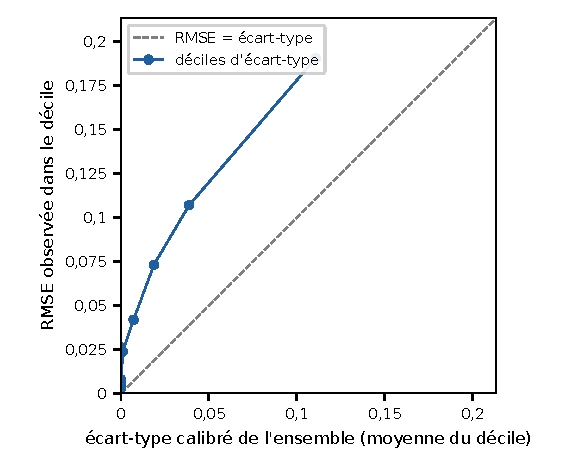
\includegraphics[width=0.62\textwidth]{calibration_incertitude.pdf}
\caption{L'incertitude suit-elle l'erreur ? RMSE observée par décile d'écart-type calibré de l'ensemble, en protocole strict (\texttt{annee2}) avec les facteurs ajustés sur le protocole inversé ; la diagonale en tirets est l'égalité entre RMSE et écart-type, et les axes sont limités à l'étendue des déciles. À partir du cinquième décile, la RMSE croît avec l'écart-type mais reste au-dessus de la diagonale (intervalles trop étroits : globalement d'un facteur 1,6, \autoref{tab:calibration}, et davantage dans les déciles intermédiaires) ; les quatre premiers déciles, d'écart-type quasi nul (circuits quasi constants, sur lesquels les cinq membres sont d'accord), ont une RMSE de 0,003 à 0,026 : un écart-type nul n'est pas une garantie.}
\label{fig:calibration}
\end{figure}

\section{Analyse des erreurs}\label{sec:erreurs}

La \autoref{fig:reve} met le rêve en face de la réalité, en moyennes journalières, pour la somme des 33~circuits et pour les quatre circuits qui pèsent le plus ; nous y lisons les trois ruptures signalées à la \autoref{sec:donnees} (extinction de NPWD2551 en janvier 2011, décrochage du 30~août 2011, allumage de février--mars 2012), que le rêve ne reproduit qu'en partie, et l'élargissement de la bande d'incertitude à ces moments. La \autoref{fig:zoom} montre, à l'échelle horaire, les cycles de NPWD2551 à l'échelle de l'orbite en saison d'éclipses ; la \autoref{fig:circuits} montre l'erreur par circuit, à côté de la constante.

\begin{figure}[htbp]
\centering
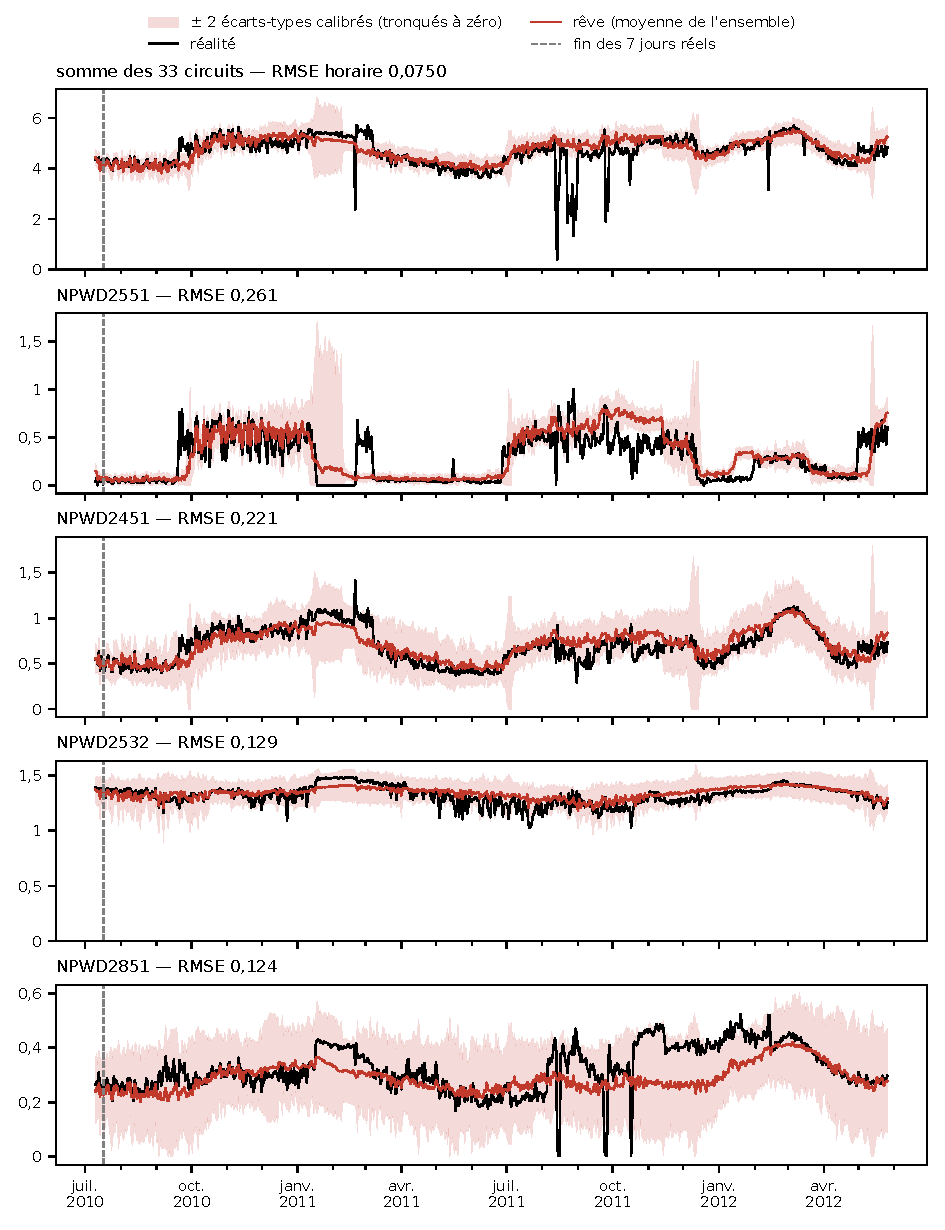
\includegraphics[width=\textwidth]{reve_vs_realite.pdf}
\caption{Rêve contre réalité en moyennes journalières, protocole strict (\texttt{annee2}, RMSE horaire 0,0750) : en haut la somme des 33~circuits, puis les quatre circuits qui pèsent le plus (NPWD2551, NPWD2451, NPWD2532, NPWD2851) avec leur RMSE. Noir : réalité ; rouge : moyenne de l'ensemble ; bande : $\pm 2$ écarts-types de l'ensemble, calibrés avec les facteurs ajustés sur l'autre année de test et tronqués à zéro ; le trait vertical en tirets marque la fin des 7~jours réels.}
\label{fig:reve}
\end{figure}

\begin{figure}[htbp]
\centering
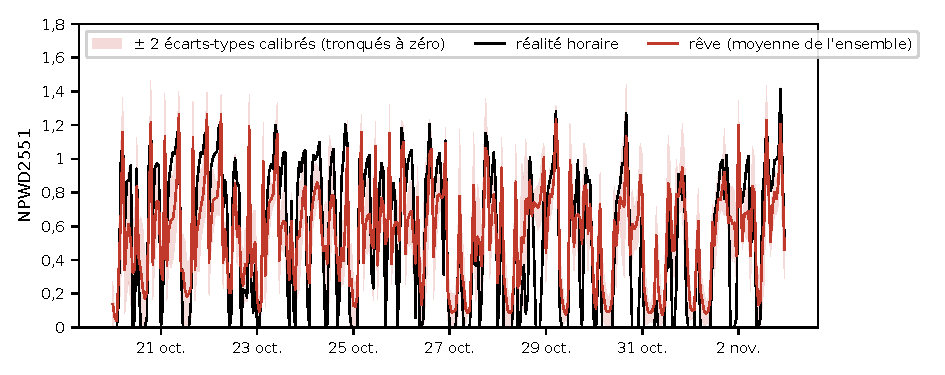
\includegraphics[width=\textwidth]{zoom_horaire.pdf}
\caption{NPWD2551 à l'échelle horaire sur deux semaines à partir du jour 95 du rêve (du 20~octobre au 2~novembre 2010 inclus, saison d'éclipses), protocole strict : réalité horaire en noir, moyenne de l'ensemble en rouge, bande à $\pm 2$ écarts-types calibrés, tronquée à zéro. Les cycles ON/OFF à l'échelle de l'orbite (environ 7\,h) sont suivis ; le rapport cyclique exact du thermostat ne l'est pas.}
\label{fig:zoom}
\end{figure}

\begin{figure}[htbp]
\centering
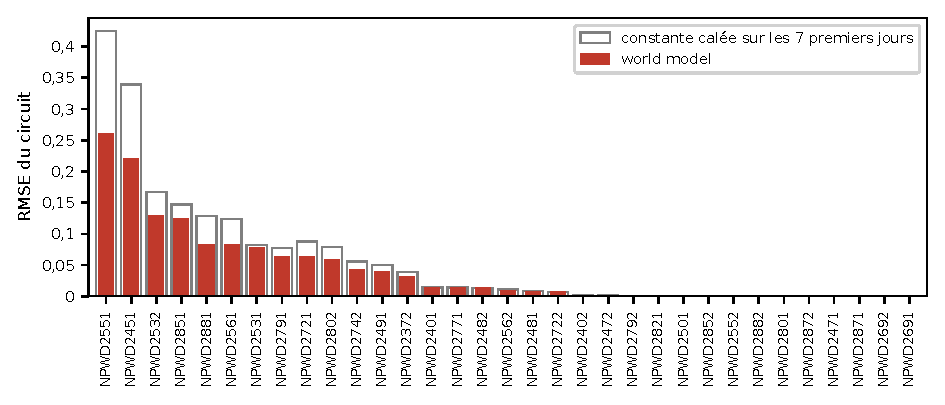
\includegraphics[width=\textwidth]{erreur_par_circuit.pdf}
\caption{RMSE par circuit en protocole strict (\texttt{annee2}), circuits triés par erreur décroissante : world model en rouge, constante calée sur les 7~premiers jours en contour gris. Les deux lignes de chauffage NPWD2551 et NPWD2451 dominent ; une quinzaine de circuits quasi constants ont une erreur négligeable.}
\label{fig:circuits}
\end{figure}

\paragraph{Deux circuits, 1,5~\% des cellules.} NPWD2551 et NPWD2451 font 63~\% de l'erreur quadratique ; 60~\% de l'erreur vient de 1,5~\% des cellules circuit $\times$ heure ($\lvert\text{erreur}\rvert > 0{,}3$) : des marches, pas du bruit. NPWD2551 est un chauffage à paliers (à zéro sur 78~\% des mesures brutes, sinon des paliers à 0,22 / 0,62 / 1,04 / 1,64 / 1,86), allumé pendant les deux saisons d'éclipses ; NPWD2451 vaut 0,05, 1,1 ou 2,16 (un ou deux éléments), sa moyenne horaire est un rapport cyclique de thermostat anticorrélé au flux solaire, autocorrélé à 0,5 seulement d'une heure à l'autre.

\paragraph{Le décrochage de 2011.} Pendant la deuxième saison d'éclipses d'\texttt{annee2} (jours 400--490), à ombre égale, NPWD2551 consomme 0,30 à 0,45 de moins qu'en \texttt{annee1} pour les heures d'umbra partiel (umbra : ombre totale de Mars, en fraction de l'heure ; 0 à 0,6), et 0,12 de plus pour les heures d'umbra pleine ; le niveau en umbra baisse dans tous les modes de pointage (INERTIAL 0,87 $\rightarrow$ 0,61, SLEW 0,89 $\rightarrow$ 0,79). D'autres lignes changent de niveau en même temps (NPWD2851 +0,11, NPWD2532 +0,18 hors ombre, NPWD2451 $-$0,11 en ombre) : la signature d'un changement de configuration thermique, pas d'un défaut de mesure. Le décrochage commence le \textbf{30~août 2011, premier jour d'un trou de 14~jours dans le fichier de commandes} (0 commande par heure, communications normales), suivi d'un trou de 35~jours à partir du 10~octobre ; cette saison contient aussi la famille de commandes AACF (0,8 commande par heure, absente d'\texttt{annee1}) et le mode de pointage D4PNPO (14~\% des heures contre 0,8~\% la même saison d'\texttt{annee1}). Un modèle entraîné sur \texttt{annee1} n'a jamais vu ni un trou de planning de plus de 15~jours, ni AACF, ni autant de D4PNPO : il n'a aucun moyen d'apprendre ce que ces heures font. Ce que le kit ne contient pas (consignes de thermostat, état réel des équipements) reste inconnu : \enquote{inexpliqué} est la conclusion exacte, pas \enquote{inexplicable}.

\paragraph{Ce que cela borne.} Un oracle qui retirerait le biais hebdomadaire de NPWD2551 seul gagnerait environ 0,004 (0,0750 $\rightarrow$ 0,0710 ; 0,0691 en corrigeant aussi NPWD2451) : la RMSE plancher avec ces entrées est vers 0,071. Le reste de l'erreur sur les deux circuits de chauffage est le rapport cyclique du thermostat, imprévisible heure par heure à partir du planning.

\paragraph{Ce qui marche.} Les saisons d'éclipses (montée et descente de NPWD2551 et NPWD2451, cycles horaires à l'échelle de l'orbite, \autoref{fig:zoom}), la saison solaire de NPWD2451, le niveau de NPWD2532 ; les lignes à deux états (NPWD2881, NPWD2561, NPWD2791) depuis que le GRU lit les comptes de commandes.

\section{Ablations}\label{sec:ablations}

Chaque ligne du \autoref{tab:ablations} réentraîne le modèle (1 graine, 80 époques, protocole strict) en retirant ou en ajoutant un ingrédient, à partir du jeu de features final. Les ablations du GRU sont mesurées sur le GRU seul (0,0802) ; la première ligne situe le système complet. Bruit entre graines : $\pm$\,0,001.

\begin{table}[htbp]
\centering\footnotesize
\caption{Ablations en protocole strict (1 graine, 80 époques) à partir du jeu de features final. L'écart est pris par rapport au GRU seul (0,0802) ; entre parenthèses, les deux circuits les plus mal prédits et leur RMSE. Bruit entre graines : $\pm$\,0,001.}
\label{tab:ablations}
\begin{tabularx}{\textwidth}{L{4.4cm} c c Y}
\toprule
Ablation & RMSE & écart & lecture \\
\midrule
\textbf{système complet : GRU + composant gradient boosting (0,5)} & 0,0751 & $-$0,005 & le GBM corrige les deux chauffages (0,28 $\rightarrow$ 0,26 ; 0,24 $\rightarrow$ 0,22) sans toucher au reste (pires : NPWD2551 0,26, NPWD2451 0,22) \\
GRU seul & 0,0802 & référence & une graine ; la moyenne de 5 graines donne 0,0796 (pires : NPWD2551 0,28, NPWD2451 0,24) \\
sans mémoire (MLP heure par heure) & 0,0818 & +0,002 & la mémoire vaut 0,002, à peine plus que le bruit de graine (pires : NPWD2551 0,28, NPWD2451 0,25) \\
sans réinjection (planning seul) & 0,0794 & $-$0,001 & relire $y_{t-1}$ n'apporte rien : la boucle d'état passe par $h_t$ (pires : NPWD2551 0,28, NPWD2451 0,24) \\
sans scheduled sampling (teacher forcing seul) & 0,0924 & +0,012 & apprendre sur ses propres sorties est ce qui tient le rêve 16\,000 pas (pires : NPWD2551 0,36, NPWD2451 0,27) \\
fenêtres indépendantes (état remis à zéro, 20 époques) & 0,0898 & +0,010 & sans état transmis, pas de régimes longs ; confondu avec 20 époques au lieu de 80 (pires : NPWD2551 0,33, NPWD2451 0,26) \\
sans éclipses ni événements (evtf) & 0,0808 & +0,001 & l'ombre est déjà dans les angles solaires et les durées d'éclipse de ltdata (pires : NPWD2551 0,29, NPWD2451 0,24) \\
sans Soleil (saaf) & 0,1004 & +0,020 & l'ingrédient n\textsuperscript{o}\,1 : NPWD2532 passe de 0,14 à 0,24, NPWD2451 de 0,24 à 0,33 (pires : NPWD2451 0,33, NPWD2551 0,30) \\
sans tendances (ltdata : constante solaire, durées d'éclipse et d'occultation) & 0,0885 & +0,008 & la saison (constante solaire, durées d'éclipse) fixe le niveau de l'année (pires : NPWD2551 0,31, NPWD2451 0,28) \\
sans pointage (ftl) & 0,0898 & +0,010 & l'attitude (quelle face au Soleil) : NPWD2551 passe de 0,28 à 0,36 (pires : NPWD2551 0,36, NPWD2451 0,25) \\
sans comptes de commandes par stem (il reste 45 features physiques) & 0,0824 & +0,002 & gain petit mais net sur les lignes à deux états : NPWD2881 entre dans les pires (pires : NPWD2551 0,29, NPWD2451 0,23) \\
avec les interrupteurs de commandes par lettre & 0,0854 & +0,005 & les lettres changent d'année : ce qu'elles font apprendre est perdu au test (pires : NPWD2551 0,31, NPWD2451 0,25) \\
avec toutes les colonnes de commandes & 0,0867 & +0,006 & des centaines de colonnes de plus : NPWD2531 (0,19) et NPWD2851 (0,17) décrochent (pires : NPWD2551 0,27, NPWD2451 0,23) \\
avec calendrier (distance Terre-Mars, angle Soleil-Mars-Terre) & 0,0888 & +0,009 & une horloge : le réseau mémorise l'année d'entraînement au lieu de la physique (pires : NPWD2551 0,34, NPWD2451 0,25) \\
\bottomrule
\end{tabularx}
\end{table}

Trois lectures. \textbf{La physique d'abord} : retirer le Soleil coûte 0,020, le pointage 0,010, les tendances 0,008, soit dix fois ce que vaut la mémoire ; les éclipses du fichier d'événements sont presque redondantes (0,001) avec les angles solaires et les durées d'éclipse journalières. \textbf{La procédure d'entraînement compte plus que l'architecture} : le scheduled sampling (0,012) et l'état transmis entre segments (0,010) sont ce qui rend une simulation de 16\,000 pas stable, alors que remplacer le GRU par un MLP coûte 0,002 et que retirer la réinjection de $y_{t-1}$ ne coûte rien : la boucle d'état est portée par $h_t$, pas par la sortie relue ; la mémoire est ce qui rend la simulation libre stable, pas ce qui prédit le niveau. C'est la limite du récit \enquote{world model}, discutée à la \autoref{sec:discussion}. \textbf{Ajouter nuit} : lettres de variante (+0,005), toutes les colonnes de commandes (+0,006), calendrier (+0,009) donnent au réseau de quoi mémoriser l'année d'entraînement au lieu d'en apprendre la physique ; le seul ajout qui paie est le compte horaire de commandes par stem (0,002, concentré sur les lignes à deux états). Enfin le composant gradient boosting vaut 0,005 sur le GRU seul, autant que le deuxième ingrédient le plus utile : deux modèles qui se trompent différemment valent mieux qu'un modèle plus gros.

\section{Application : comparaison de plannings alternatifs}\label{sec:pilote}

Le world model sert de simulateur pour comparer des plannings sur 14~jours en saison d'éclipses, à partir du 25~octobre 2010, initialisés par les 7~jours réels précédents, avec le modèle entraîné sur \texttt{annee1} seule. Les fenêtres de communication avec la Terre ne sont jamais touchées ; après chaque modification du planning, les features dérivées (anticipation, inertie) sont recalculées. \textbf{Comparaison appariée} : chaque membre de l'ensemble simule le planning réel et le planning modifié ; nous rapportons la moyenne des différences, leur dispersion entre membres et l'accord des membres sur le signe. C'est l'incertitude du modèle sur la différence, bien plus petite que celle sur le niveau (dispersion entre membres de $\pm$\,10,2 sur une consommation cumulée de 1\,728, soit $\pm$\,0,6~\%). La grandeur comparée est la consommation cumulée : la somme des 33~valeurs horaires sur les 14~jours, dans la même unité que la télémétrie (\autoref{tab:pilote}).

\begin{table}[htbp]
\centering\small
\caption{Comparaison de plannings : consommation cumulée simulée (somme des 33~valeurs horaires sur 14~jours à partir du 25~octobre 2010, même unité que la télémétrie) pour le planning réel et quatre plannings modifiés, en comparaison appariée sur les cinq membres de l'ensemble.}
\label{tab:pilote}
\begin{tabularx}{\textwidth}{Y C{2.4cm} C{2.6cm} C{2.2cm} C{1.7cm}}
\toprule
Planning & consommation cumulée simulée & écart & dispersion entre membres & membres d'accord \\
\midrule
Réel (mesuré : 1\,726,2) & 1\,728,4 & référence (+0,1~\% du réel) & & \\
Hors communication, tout en pointage EARTH (plus d'observation) & 1\,717,6 & $-$0,62~\% & $\pm$\,0,07~\% & 5/5 \\
Hors communication, tout en NADIR (observation continue) & 1\,718,0 & $-$0,60~\% & $\pm$\,0,26~\% & 5/5 \\
Hors communication, sans manœuvres (SLEW rendu à EARTH) & 1\,724,9 & $-$0,20~\% & $\pm$\,0,03~\% & 5/5 \\
\textbf{Recherche locale} : permutations d'heures de pointage dans chaque journée, 120 essais, 15 gardées & 1\,727,6 & $-$0,05~\% & $\pm$\,0,01~\% & 5/5 \\
\bottomrule
\end{tabularx}
\end{table}

Lecture : le chauffage dépend d'abord de la physique (ombre, Soleil), pas du planning ; les écarts sont de l'ordre du pour cent au plus. Le gain \enquote{facile} (tout en EARTH) consiste à ne plus observer, ce qui n'est pas un planning acceptable. La recherche locale ne retire aucune observation : elle déplace des heures de pointage à l'intérieur de chaque journée et ne garde une permutation que si les cinq membres la jugent favorable ; elle trouve $-$0,05~\% en 120 essais (15 permutations gardées), un gain cohérent entre membres mais près de trois fois plus petit que l'écart entre le planning réel simulé et le réel mesuré (+0,1~\%). Rien de tout cela n'est vérifiable : ces plannings n'ont pas volé. L'application mesure ce que le modèle croit, et la comparaison appariée dit seulement si le modèle est sûr de lui.

\section{Discussion et limites}\label{sec:discussion}

Le récit \enquote{world model} est plus ambitieux que ce que les ablations soutiennent : la mémoire vaut 0,002, la réinjection de l'état rien, et les 7~jours réels n'informent que la première semaine. Le problème, tel que les données le posent, est une régression contextuelle avec une contrainte de stabilité sur 16\,000 pas, et c'est ce que le système fait. Trois enseignements du journal des essais (\annexeref{app:journal}) vont dans le même sens. Le GRU a atteint un plateau dès les premiers essais : aucune variante d'architecture ou d'optimisation (LSTM, 256 neurones, deux couches, moyenne stochastique des poids, perte de Huber, réglage du dropout, du bruit ou du taux d'apprentissage) ne l'a déplacé de plus que le bruit de graine. Les lettres de variante des commandes, qui changent d'une année martienne à l'autre, ont été le piège principal : tout ce qui est appris par lettre est perdu l'année suivante, et seuls les événements sans lettre (comptes par stem, changements de variante) sont stables. Enfin l'empilement a été battu par le simple mélange (\autoref{sec:modele}).

Les limites tiennent d'abord aux données. Il n'y a qu'une année de test par sens : deux protocoles sur deux années sont le maximum que le kit permet ; l'optimisme de sélection résiduel est de l'ordre du millième, mais une troisième année, avec de nouveaux régimes, peut sortir de la fourchette 0,0805--0,0901, qui est la seule estimation honnête de la RMSE du modèle final entraîné sur les deux années. Ce qui n'est pas dans le kit ne peut pas être appris : consignes de thermostat, trous de planning de 35~jours, familles de commandes nouvelles ; une troisième année martienne de données compterait sans doute plus que n'importe quel modèle, mais l'appui chiffré est faible : le gradient boosting à toutes les colonnes de l'\annexeref{app:journal} passait de 0,089 à 0,082 avec une demi-année d'entraînement de plus, sur une période de test différente, et le GBM final, lui, n'y gagne rien (0,0792 en strict contre 0,0816 en chronologique). L'incertitude calibrée est une échelle, pas une loi : elle est juste en moyenne par circuit, pas heure par heure, parce que les erreurs sont des marches, pas des gaussiennes. Enfin l'application de pilotage est une démonstration d'usage, pas un résultat : ses écarts sont de l'ordre du pour cent et invérifiables.

\section{Conclusion}\label{sec:conclusion}

Nous avons construit un simulateur heure par heure de la consommation de 33~circuits de Mars Express sur une année martienne entière : un ensemble de cinq GRU entraînés pour la simulation libre, mélangé à parts égales avec un composant gradient boosting en bagging temporel. Dans les trois protocoles de validation chronologiques, dont un ajouté après toutes les décisions de conception, il obtient 0,0750, 0,0901 et 0,0805 de RMSE, soit 23 à 29~\% de moins qu'une prédiction constante, et le mélange bat chacune de ses composantes. Les ablations établissent la hiérarchie des ingrédients : la physique (Soleil, pointage, saison) fait l'essentiel de la prédiction, la procédure d'entraînement (état transmis entre segments, scheduled sampling) compte plus que l'architecture, et les ajouts qui donnent au réseau de quoi mémoriser l'année d'entraînement (lettres de variante, calendrier) nuisent. L'erreur restante est concentrée : deux lignes de chauffage à thermostat, 1,5~\% des cellules, et un décrochage de 2011 que le planning n'explique pas. L'incertitude de l'ensemble, calibrée d'une année de test sur l'autre, classe les heures incertaines sans encore les quantifier. Ce qu'il faudrait ensuite n'est pas un modèle plus gros, mais une troisième année martienne de données et des informations que le kit ne contient pas : consignes de thermostat et état réel des équipements.

\section*{Disponibilité du code}

Le code est disponible à l'adresse \url{https://github.com/kenzi0228/dream-in-orbit}. Il repose sur PyTorch \citep{paszke2019pytorch} et scikit-learn \citep{pedregosa2011scikit}, avec des versions épinglées (torch 2.2.2, scikit-learn 1.6.1, pandas 2.3.3, numpy 1.26.4, pyarrow 21.0.0, matplotlib 3.9.4), et a été testé avec Python 3.9 sur macOS, sur CPU uniquement. Les commandes qui reproduisent chaque résultat, les trois protocoles et l'organisation du code sont en \annexeref{app:repro}.

\section*{Remerciements}

Nous remercions les organisateurs de l'épreuve Dream in Orbit pour le kit de données et son script d'évaluation, et l'Agence spatiale européenne, dont la télémétrie de Mars Express est à l'origine de ces données.

% La bibliographie est composée en anglais : titres anglais et identifiants (arXiv:…, doi:…) sans espace
% automatique avant « : » ; otherlanguage* ne change pas les légendes, le titre reste « Références ».
\begin{otherlanguage*}{english}
\bibliographystyle{plainnat}
\bibliography{references}
\end{otherlanguage*}

\appendix
% titres d'annexes « Annexe A  Essais négatifs » (les annexes n'ont pas de sous-sections numérotées)
\makeatletter
\renewcommand{\@seccntformat}[1]{Annexe~\csname the#1\endcsname\quad}
\makeatother

\section{Journal des essais (résultats négatifs compris)}\label{app:journal}

Tout ce qui suit a été mesuré dans les protocoles strict et chronologique (fichiers \texttt{experiments.csv}, \texttt{gbm\_*.json} et \texttt{reblend\_*.json} du dossier \texttt{reports/} du dépôt) ; seuls les résultats utiles au lecteur sont gardés. Les paires de chiffres se lisent strict / chronologique.

\paragraph{Première passe : apprendre à rêver.} Un GRU en teacher forcing pur dérive en quelques jours de simulation (0,13) ; le scheduled sampling et l'entraînement par flux continus le ramènent à 0,088. Les features de calendrier (distance Terre-Mars, angle Soleil-Mars-Terre) font mémoriser l'année d'entraînement : les retirer donne 0,083. Les 77 états d'interrupteurs de commandes par lettre font tomber le GRU à 0,103 (strict) et 0,121 (chronologique). Le GRU \enquote{physique} (47 features) atteint 0,0821 / 0,0901.

\paragraph{Deuxième passe : le plateau du GRU, puis un second modèle.} Aucune variante seule ne déplace le GRU physique de plus que le bruit : LSTM 0,0825, 256 neurones 0,0836, 2 couches 0,0835 (0,0993 en chronologique), moyenne stochastique des poids (SWA) 0,0832, perte de Huber 0,0825--0,0837, dropout / bruit / taux d'apprentissage / weight decay 0,082--0,083 ; adaptation au test sur les 7~jours réels 0,084 $\rightarrow$ 0,104 (surapprend une semaine) ; mémoire thermique explicite, flux par face, anticipation $t \pm 3$ : dans le bruit ou pire en chronologique. Deux GRU de graines différentes ont des erreurs corrélées à 0,96--0,99 : les moyenner n'apporte rien. Un gradient boosting heure par heure sur toutes les colonnes est moins bon seul (0,0891) mais corrélé à 0,75 seulement : mélangé à 0,45, 0,0779 / 0,0830. ExtraTrees et RandomForest en plus : rien ; poids de mélange par circuit : surapprennent la période de validation (choisis sur un protocole, pires sur l'autre) ; second GRU sur toutes les features : rien de plus une fois le GBM présent.

\paragraph{Troisième passe : les lettres.} L'erreur décomposée (deux circuits, 1,5~\% des cellules, \autoref{sec:erreurs}) et une découverte : les lettres de variante des commandes changent d'une année à l'autre (20 interrupteurs sur 29, 7 sans aucune lettre commune, 49 commandes du vocabulaire présentes seulement en \texttt{annee2}). Tout ce qui est appris par lettre est perdu l'année suivante ; aucun encodage sans lettre de l'\textbf{état} d'un interrupteur n'est stable (rang d'apparition, parité, variante majoritaire : tous s'inversent). Les \textbf{événements} le sont : comptes par stem, changements de variante à venir et passés. GBM sans aucune lettre + ces features : 0,0822 / 0,0829 contre 0,0891 / 0,0823 ; bagging temporel en 5 sacs : 0,0796 / 0,0820 ; GRU + comptes par stem : 0,0795 / 0,0901 (première amélioration du GRU depuis la première semaine), alors que les récences par stem (0,1029) et les changements d'interrupteurs (0,0920) lui nuisent : des rampes de plusieurs semaines sont des horloges. Négatifs : moyennes exponentielles pour le GBM (0,0909 / 0,0866), pondération des données récentes (0,0827--0,0836 contre 0,0823), mélange pondéré par l'incertitude (différence de 0,0003, dans le bruit), projection de rang faible, 7 ou 31 feuilles (0,0803 / 0,0849 et 0,0845 / 0,0824 : le compromis est 15), 161 stems au lieu de 115--149 (GRU 0,0810 / 0,0925). Système : 0,0751 / 0,0808.

\paragraph{Quatrième passe : la méthode.} Vocabulaire appris sur l'entraînement seul (le strict passe de 0,07509 à 0,0750 avec cinq graines : la fuite de noms de colonnes ne valait rien, mais elle existait) ; protocole inversé comme année de test vierge ; empilement essayé et battu (GRU lisant le GBM hors-échantillon et apprenant le résidu : 0,0908 ; résidu seul : 0,0884 ; contre 0,0751 pour le mélange à une graine, explication à la \autoref{sec:modele}) ; calibration de l'incertitude par circuit, vérifiée d'une année sur l'autre ; application de pilotage en comparaison appariée ; diagnostic du décrochage de 2011 ; test de bout en bout de l'entraînement à la prédiction ; cache du GBM pour que les relances et les ablations ne le réajustent pas ; poids du GBM compressés (45\,Mo au lieu de 206).

\section{Reproductibilité : commandes et organisation du code}\label{app:repro}

Le kit doit se trouver dans \texttt{kit\_etudiants/} (\texttt{annee1/}, \texttt{annee2/}, \texttt{make\_validation.py}, \texttt{evaluate.py}).

\paragraph{Installation.}
{\small
\begin{verbatim}
python3 -m venv .venv
.venv/bin/pip install -r requirements.txt
\end{verbatim}
}

\paragraph{Entraînement et prédiction.} \texttt{train.py} entraîne tout (\texttt{annee1} + \texttt{annee2}) en une commande et écrit les poids dans \texttt{weights/} (environ 70\,min sur 6~cœurs) ; \texttt{predict.py} est l'interface officielle et simule une période de test au format de l'évaluation, avec l'incertitude calibrée en option.
{\small
\begin{verbatim}
.venv/bin/python train.py
.venv/bin/python predict.py --test_dir DOSSIER --out predictions.csv \
    [--std_out incertitude.csv]
\end{verbatim}
}

\paragraph{Validation dans les conditions exactes de l'évaluation.} Entraînement sur \texttt{annee1} seulement, poids dans \texttt{weights\_holdout/}, puis flux officiel :
{\small
\begin{verbatim}
.venv/bin/python train.py --holdout
cd kit_etudiants
../.venv/bin/python make_validation.py --annee annee2 --out ../validation
cd ..
.venv/bin/python predict.py --test_dir validation/test --out pred.csv \
    --weights weights_holdout
.venv/bin/python kit_etudiants/evaluate.py --pred pred.csv \
    --verite validation/verite_horaire.csv \
    --heures validation/test/heures_a_predire.csv
\end{verbatim}
}
\texttt{train.py --holdout-reverse} (\texttt{annee2} $\rightarrow$ \texttt{annee1}) et \texttt{train.py --holdout-split 0.5} (deux ans $\rightarrow$ $\tfrac{1}{2}$~\texttt{annee2}) sont les deux autres protocoles du rapport ; \texttt{train.py --combine none} donne la version réseau de neurones pur et \texttt{--gbm-weight} règle le poids du composant gradient boosting.

\paragraph{Reproduire le rapport.} Une commande relance toute la chaîne de livrables, soit, dans l'ordre : les trois validations, le flux officiel, la calibration, le modèle final, la démo, l'application de pilotage, les ablations, les tableaux du rapport, le diagnostic de NPWD2551 et les tests (environ 4\,h sur 6~cœurs, le GBM étant mis en cache) :
{\small
\begin{verbatim}
./run_all.sh 6
\end{verbatim}
}
Chaque étape est aussi une commande seule (\autoref{tab:code}). Les tests (features, puis chaîne complète de \texttt{train.py} à \texttt{predict.py}) se lancent par
{\small
\begin{verbatim}
.venv/bin/python tests/test_features.py
.venv/bin/python tests/test_predict_smoke.py
\end{verbatim}
}
Le modèle final dans \texttt{weights/} (5 fichiers \texttt{model\_k.pt}, 3\,Mo ; \texttt{gbm.pkl}, le composant gradient boosting compressé, 45\,Mo ; \texttt{meta.json}, vocabulaire et liste des features ; \texttt{calibration.json}) est entraîné sur \texttt{annee1} + \texttt{annee2}. Les figures de ce rapport sont produites par \texttt{rapport/figures.py} à partir des mêmes fichiers que \texttt{demo.py}.

\begin{table}[htbp]
\centering\small
\caption{Organisation du code.}
\label{tab:code}
\begin{tabularx}{\textwidth}{l Y}
\toprule
Fichier & Contenu \\
\midrule
\texttt{train.py} & entraînement en une commande ; protocoles \texttt{--holdout}, \texttt{--holdout-reverse}, \texttt{--holdout-split} ; \texttt{--combine blend}, \texttt{none} ou \texttt{stack} \\
\texttt{predict.py} & interface officielle (+ \texttt{--std\_out}, incertitude calibrée) \\
\texttt{calibrate.py} & facteurs d'échelle de l'incertitude par circuit, ajustés sur une validation, vérifiés sur les autres \\
\texttt{dio/features.py} & alignement des 5 fichiers de contexte sur la grille horaire, vocabulaire appris sur l'entraînement (fiches de l'annexe~\ref{app:fiches}) \\
\texttt{dio/data.py} & chargement avec cache (\texttt{cache/}), groupes de features \\
\texttt{dio/model.py} & le world model GRU (teacher forcing, rollout avec scheduled sampling), normalisation \\
\texttt{dio/gbm.py} & le composant gradient boosting (sacs temporels, prédictions hors-échantillon, cache) \\
\texttt{dio/simulate.py} & simulation d'une période avec l'ensemble (membres, moyenne, écart-type) \\
\texttt{dio/metrics.py} & RMSE identique à \texttt{evaluate.py}, par circuit, par horizon \\
\texttt{baselines.py} & constante, persistance, gradient boosting heure par heure \\
\texttt{ablations.py} & réentraîne le GRU sans tel ou tel ingrédient (\texttt{reports/ablations.md}) \\
\texttt{demo.py} & figures \enquote{rêve contre réalité}, dérive, erreur par circuit, calibration (\texttt{reports/figures/}) \\
\texttt{pilot.py} & application : comparaison appariée de plannings alternatifs (\texttt{reports/pilot.json}) \\
\texttt{experiments/} & harnais d'expériences et analyses (voir \texttt{experiments/README.md}) \\
\texttt{tests/} & tests unitaires des features et test de bout en bout \texttt{train.py} $\rightarrow$ \texttt{predict.py} \\
\texttt{run\_all.sh} & relance toute la chaîne de livrables (environ 4\,h sur 6~cœurs) \\
\texttt{rapport/} & sources LaTeX de ce rapport et \texttt{figures.py}, qui produit ses figures \\
\bottomrule
\end{tabularx}
\end{table}

\clearpage
\section{Fiches détaillées des six fichiers du kit}\label{app:fiches}

Une fiche par fichier (tableaux \ref{tab:power} à \ref{tab:ltdata}) : volume, format, vocabulaire appris sur l'entraînement, features dérivées avec les préfixes de colonnes du dépôt, liens physiques et pièges. Le \autoref{tab:kit} en est le résumé.

\begin{table}[htbp]
\centering\small
\caption{Fiche du fichier power.csv, l'état : volume, valeurs, circuits qui pèsent dans la RMSE, comportement des lignes de chauffage et changements de régime.}
\label{tab:power}
\begin{tabularx}{\textwidth}{>{\bfseries\raggedright\arraybackslash}p{3.1cm} Y}
\toprule
Lignes & 1,83 million (\texttt{annee1}), 1,77 million (\texttt{annee2}), soit une mesure toutes les $\approx$\,32\,s \\
Valeurs & courant moyen par circuit, de 0 à $\approx$\,2,2, en unités du fichier (le kit ne précise pas l'unité) ; 13 à 17 circuits selon l'année sont quasi constants (écart-type $<$ 0,001) \\
Qui pèse dans la RMSE & NPWD2551 (36~\% de l'erreur quadratique de la constante), NPWD2451 (25~\%), NPWD2851 (9~\%), NPWD2532 (9~\%), NPWD2531 (5~\%), NPWD2881 (4~\%) \\
Comportement & NPWD2551 et NPWD2451 sont des lignes de chauffage à thermostat : fortes pendant les saisons d'éclipses (moyenne 0,5--0,8 contre 0,03--0,1 hors saison), cycles ON/OFF à l'échelle de l'orbite (7\,h), autocorrélation à 1\,h $\approx$ 0,6 seulement \\
Pièges & changements de régime d'une année à l'autre : NPWD2531 passe de 0,4--0,6 (automne 2008) à $\approx$\,0 ensuite ; NPWD2551 s'éteint en janvier 2011 malgré les éclipses, décroche le 30~août 2011 (\autoref{sec:erreurs}) et s'allume en février--mars 2012 sans éclipse \\
\bottomrule
\end{tabularx}
\end{table}

\begin{table}[htbp]
\centering\small
\caption{Fiche du fichier dmop.csv, les commandes (actions) : volume, format des commandes, vocabulaire appris sur l'entraînement, features dérivées sans lettre de variante et pièges (dérive du vocabulaire, trous).}
\label{tab:dmop}
\begin{tabularx}{\textwidth}{>{\bfseries\raggedright\arraybackslash}p{3.1cm} Y}
\toprule
Lignes & 187\,000 (\texttt{annee1}), 144\,000 (\texttt{annee2}) ; instant (ms UTC) + nom de commande \\
Format & \texttt{AAAAF56A1} : 4 lettres de sous-système (AAAA, APSF, AMMM, ATTT = thermique, AXXX\ldots), un code, une lettre de variante. Les entrées \texttt{MAPO.000\ldots}/\texttt{MPER.\ldots} marquent apocentre/péricentre, \texttt{PENS}/\texttt{PENE}, \texttt{MOCS}/\texttt{MOCE}\ldots\ sont des paires début/fin \\
Vocabulaire & 9\,280 commandes distinctes dans \texttt{annee1} ; le vocabulaire des features est appris sur la période d'entraînement seule (\autoref{sec:protocole}) : en strict, 148 commandes fréquentes, 117 \enquote{stems} (commande sans sa lettre de variante) émis $\geq$ 50 fois, 18 interrupteurs (stems à plusieurs variantes fréquentes, 49 couples stem/lettre) sur les 29 observés sur les deux années réunies \\
Features retenues & \textbf{sans lettre de variante} : comptes horaires par stem (\texttt{dm\_sc\_}), commandes à venir dans l'heure et les 6 heures suivantes (\texttt{dm\_sn1\_}, \texttt{dm\_sn6\_}), heures depuis / jusqu'au prochain changement de variante de chaque interrupteur (\texttt{dm\_sw\_}), comptes par sous-système, récences par sous-système et par stem, fraction d'heure dans les intervalles début/fin. Les features par lettre (\texttt{dm\_s\_} états, \texttt{dm\_c\_} comptes, \texttt{dm\_r\_} récences par commande) existent dans le cache mais aucun modèle final ne les lit \\
Pièges & dérive du vocabulaire d'une année à l'autre : les lettres de variante changent pour 20 des 29 interrupteurs, le sous-système AACF (5\,825 commandes) n'existe que dans \texttt{annee2} ; \textbf{trous} de plus de 24\,h : le fichier est vide 126~jours dans \texttt{annee2} (huit trous de 7 à 35~jours, dont deux de 34 et 35~jours, un de 14 et un de 15) contre 56~jours dans \texttt{annee1} (sept trous, aucun de plus de 15~jours) \\
\bottomrule
\end{tabularx}
\end{table}

\begin{table}[htbp]
\centering\small
\caption{Fiche du fichier ftl.csv, les pointages (actions) : volume, types de pointage et features dérivées.}
\label{tab:ftl}
\begin{tabularx}{\textwidth}{>{\bfseries\raggedright\arraybackslash}p{3.1cm} Y}
\toprule
Lignes & 19\,600 / 20\,000 intervalles (début, fin) avec un type et un drapeau de communication \texttt{flagcomms} \\
Types & EARTH (59~\% du temps), SLEW (14~\%), INERTIAL, MAINTENANCE, NADIR, WARMUP, RADIO\_SCIENCE, ACROSS\_TRACK, D4PNPO\ldots\ (16 types) ; D4PNPO couvre 658 heures d'\texttt{annee1} et 1\,958 d'\texttt{annee2} \\
Features & fraction d'heure dans chaque type, fraction avec communication (\texttt{ftl\_comms}, 28~\% du temps), nombre de changements de pointage dans l'heure \\
\bottomrule
\end{tabularx}
\end{table}

\begin{table}[htbp]
\centering\small
\caption{Fiche du fichier saaf.csv, les angles du Soleil (contexte) : volume, colonnes, features dérivées et lien physique avec le chauffage.}
\label{tab:saaf}
\begin{tabularx}{\textwidth}{>{\bfseries\raggedright\arraybackslash}p{3.1cm} Y}
\toprule
Lignes & 1,26 million / 1,31 million, une mesure toutes les $\approx$\,47\,s ; \texttt{sa} (aspect solaire), \texttt{sx}, \texttt{sy}, \texttt{sz} (angles avec les axes) \\
Features & moyenne horaire des 4 angles et de leurs cosinus, écart-type horaire de \texttt{sa} ; trous comblés par interpolation \\
Lien physique & hors saison d'éclipses, NPWD2551 passe de 0,09 (\texttt{sa} $\leq$ 2\textdegree) à 0,3--0,46 (\texttt{sa} $>$ 20\textdegree) : moins de Soleil sur la face chauffée $\rightarrow$ plus de chauffage \\
\bottomrule
\end{tabularx}
\end{table}

\begin{table}[htbp]
\centering\small
\caption{Fiche du fichier evtf.csv, les événements orbitaux (contexte) : volume, types d'événements, features dérivées et lien physique avec le chauffage.}
\label{tab:evtf}
\begin{tabularx}{\textwidth}{>{\bfseries\raggedright\arraybackslash}p{3.1cm} Y}
\toprule
Lignes & 76\,800 / 75\,200 ; \texttt{MAR\_UMBRA\_START/END}, \texttt{MAR\_PENUMBRA\_\ldots}, \texttt{OCC\_MARS\_\ldots}, \texttt{PERICENTRE\_PASSAGE}, \texttt{APOCENTRE\_PASSAGE}, \texttt{800/1200/2000/4000\_KM\_ASCEND/DESCEND}, \texttt{XXX\_AOS/LOS} (stations sol) \\
Features & fraction d'heure en ombre (umbra, pénombre, ombre de Phobos/Deimos), en occultation, en contact station ; temps depuis / jusqu'au péricentre, phase orbitale (cos, sin), log de l'altitude interpolée (péricentre $\approx$ 330\,km, apocentre $\approx$ 10\,100\,km) \\
Lien physique & en saison d'éclipses, NPWD2551 vaut 0,73--0,84 dans l'heure de l'umbra contre 0,35--0,55 ensuite \\
\bottomrule
\end{tabularx}
\end{table}

\begin{table}[htbp]
\centering\small
\caption{Fiche du fichier ltdata.csv, les tendances journalières (contexte) : colonnes, interpolation et piège du calendrier déguisé.}
\label{tab:ltdata}
\begin{tabularx}{\textwidth}{>{\bfseries\raggedright\arraybackslash}p{3.1cm} Y}
\toprule
Lignes & 687 / 687, une par jour : distances Soleil-Mars et Terre-Mars, angle Soleil-Mars-Terre, constante solaire, durée d'éclipse et d'occultation \\
Features & interpolation linéaire à l'heure \\
Piège & \textbf{distance Terre-Mars et angle Soleil-Mars-Terre jouent le rôle de calendrier} : leur période (780\,j) diffère de l'année martienne (687\,j), donc le couple (distance Soleil-Mars, distance Terre-Mars), de périodes 687 et 780\,j, identifie la date de façon unique. Un réseau les utilise pour mémoriser l'année d'entraînement : nous les retirons (ablation : +0,009, \autoref{tab:ablations}) \\
\bottomrule
\end{tabularx}
\end{table}

\end{document}
